\section{Team Based Learning}

Nesta seção, será descrito os conceitos-chave relacionado à metodologia ativa de aprendizagem TBL.

\subsection{O que é o TBL?}

De acordo com \cite{burgess} o TBL é uma estratégia educacional para grandes classes que, a partir coordenação do professor, possibilita a interação e colaboração em pequenos grupos centrados no estudante para melhorar o processo de aprendizagem e capacitar os alunos para o mercado. Ele foi desenvolvido para cursos de administração nos anos de 1970, por Larry Michaelsen \cite{sweet}. Os estudos de Thompson, et al (citado por \citeauthor{matalonga}, \citeyear{matalonga}) mostrou que o TBL foi inicialmente usado em medicina e desde então foi implementado em cursos de engenharia.

No TBL, os pequenos grupos trabalham juntos promovendo o aprendizado ativo e efetivo ao longo do semestre, resolvendo problemas, discutindo e aplicar conceitos inicialmente aprendidos através de leituras individuais \cite{gomez}. O aprendizado em pequenos grupos produz maiores conquistas e relacionamentos mais saudáveis e mais positivos entre alunos, do que relacionamentos competitivos ou experiências individuais (Johnson, Johnson e Smith, citado por \citeauthor{gomez}, \citeyear{gomez}).

Na sala de aula, a TBL pode ajudar a melhorar a percepção dos alunos sobre a forma como as aulas são realizadas, aumentar a compreensão dos alunos sobre os assuntos que estudam, e até mesmo ajudá-los a melhorar suas notas (Letassy et al, Anwar et al, Vasan at al, citado por \citeauthor{cabrera}, \citeyear{cabrera}).

De acordo com \cite{sweet} o TBL é uma implementação estruturada de uma abordagem de aprendizagem ativa, regida por quatro princípios:

\begin{enumerate}
  \item \textbf{Os grupos devem ser devidamente formados e gerenciados}: Todo o processo de aprendizagem é realizado em torno da formação e interação de indivíduos em pequenas equipes permanentes e diversificadas.
  \item \textbf{Os alunos devem ser responsáveis pelo qualidade do seu trabalho}: O TBL deve promover a noção de que os alunos devem ser responsáveis pelo seu aprendizado e pela qualidade de seu trabalho.
  \item \textbf{As atividades da equipe na classe devem promover o aprendizado e o desenvolvimento da equipe}: Essas atividades devem promover a discussão e a tomada de decisões.
  \item \textbf{Os alunos devem receber comentários frequentes e imediatos}: O feedback é essencial para o aprendizado e a retenção do conhecimento.
\end{enumerate}

Ao aderir aos quatro elementos essenciais acima, os professores criam um contexto que promove a quantidade e a qualidade da interação necessária para transformar os grupos em equipes de aprendizagem altamente eficazes. Além disso, ao longo do tempo, a confiança dos alunos em suas equipes cresce até o ponto em que eles estão dispostos e capazes de enfrentar tarefas difíceis com pouca ou nenhuma ajuda externa \cite{sweet}.

A organização de uma atividade utilizando o TBL é definida nas seguintes etapas: Primeiro deve ser formado as equipes.  Os grupos devem ser compostos de cinco a sete integrantes e deve ser formado de forma diversificada, oferecendo os recursos necessários. São fatores dificultadores à coesão do grupo: vínculos afetivos entre os membros, expertise diferenciada, entre outros \cite{bollela}. De acordo com Hyrnchak e Batty (citado por \citeauthor{bollela}, \citeyear{bollela}) a tarefa de formação dos grupos devem ser realizadas somente pelo professor. Após isso deve ser realizada as etapas propostas pelo TBL.

Cada módulo, unidade de trabalho ou tema coerente dentro do curso, segue um processo de aprendizagem iterativo que repete uma sequência de atividades propostas pelo TBL especificado na figura \ref{fig:tbl1} \cite{bollela}:

\begin{enumerate}
  \item \textbf{Preparação individual} através de leitura fora da classe dos materiais disponibilizados.
  \item \textbf{Avaliação de prontidão ou garantia de preparo} (RAT – \textit{Readiness Assurance Test}) através de testes individuais  (iRAT) e em equipe (gRAT). Nesta etapa, as atividades desenvolvidas buscam checar e garantir que o estudante está preparado e pronto para resolver testes individualmente, para contribuir com a sua equipe e aplicar os conhecimentos na etapa seguinte do TBL. Nesta etapa também é aplicado a apelação caso algum aluno se oponha ao resultado da avaliação.
  \item \textbf{Aplicação dos conhecimentos} (conceitos) adquiridos pela equipe por meio da resolução de problemas reais, essa atividade deve ocupar a maior parte do tempo.
  \item \textbf{Avaliação em pares} (opcional) para avaliar o desempenho de cada membro da equipe.
\end{enumerate}

\begin{figure}[h!]
	\centering
  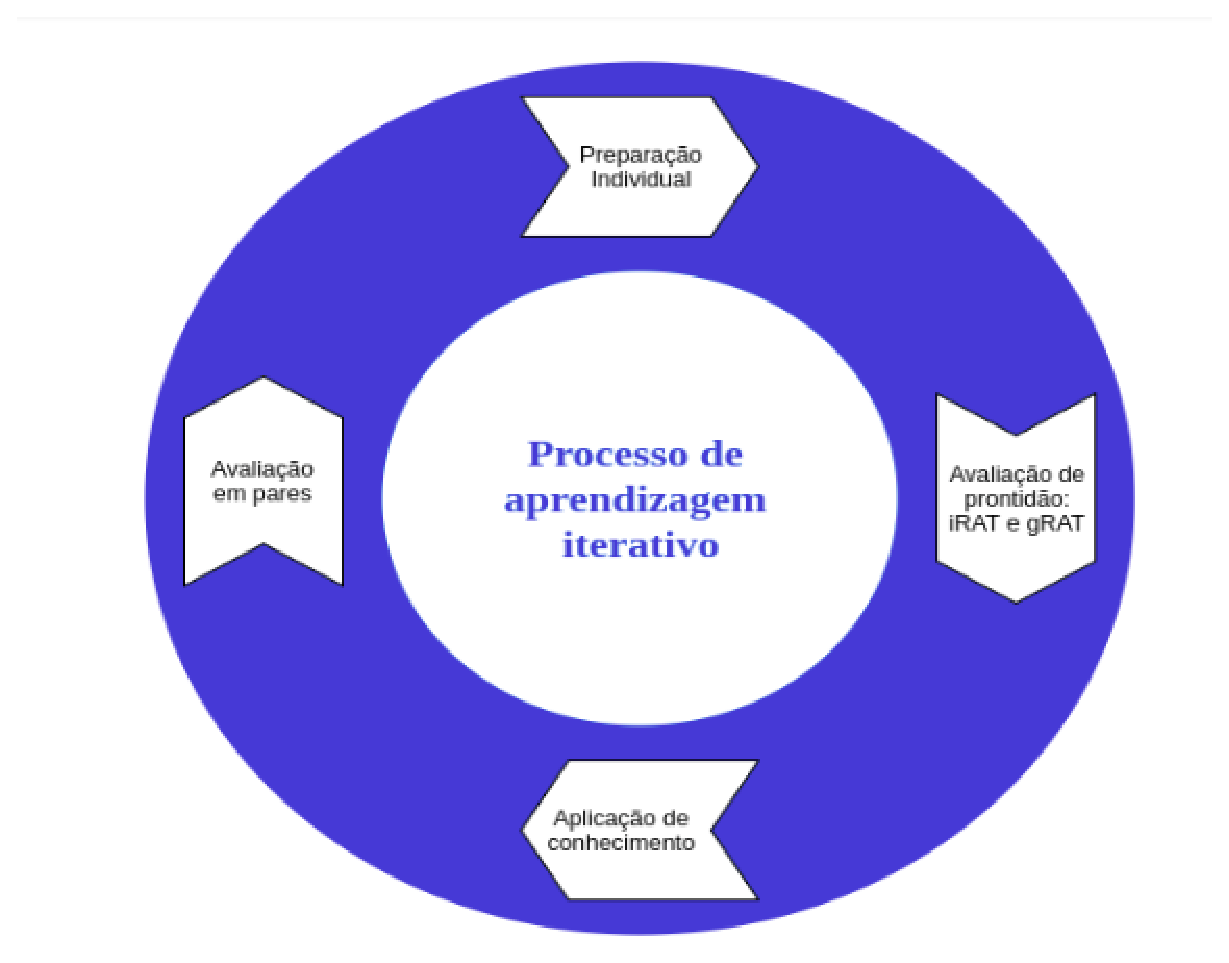
\includegraphics[keepaspectratio=true,scale=0.5]{figuras/tbl1.eps}
  \caption{Team-Based Learning processo iterativo.}
	\label{fig:tbl1}
\end{figure}

Para \cite{bollela} um aspecto crítico para implantar o TBL é a colaboração dos alunos dentro dos grupos. É importante que os membros da equipe busquem uma boa interação para que não haja conflitos. A intervenção do professor-facilitador deve ser adiada o máximo possível, permitindo que o próprio grupo busque a solução de seus problemas principalmente na etapa de aplicação de conceitos. Ele deve desenvolver questões ou testes que exijam das equipes uma resposta ("um produto") que possa ser facilmente observada e comparada entre as equipes e com possibilidade de incluir a perspectiva do especialista. Por isso a aplicação de apenas algumas etapas do TBL é alvo de críticas de seus criadores \cite{sweet}. Embora customizações sejam inevitáveis, é necessário ter a clareza de que, com isto, nem todos os benéficos atributos da metodologia serão alcançados.

A etapa de aplicação do conhecimento deve ser estruturada seguindo alguns preceitos. Os quatro princípios básicos para elaborar esta fase são conhecidos em inglês como os 4 S’s: Problema significativo e real (\textit{Significant}), O mesmo problema para todas as equipes (\textit{Same}), Respostas curtas e específicas (\textit{Specific}) e Relatos simultâneos (\textit{Simultaneous report}), ou seja, as respostas devem ser mostradas simultaneamente, de modo a inibir que alguns grupos manifestem sua resposta a partir da argumentação de outras equipes \cite{bollela}.

Em resumo temos:

\begin{figure}[h!]
	\centering
  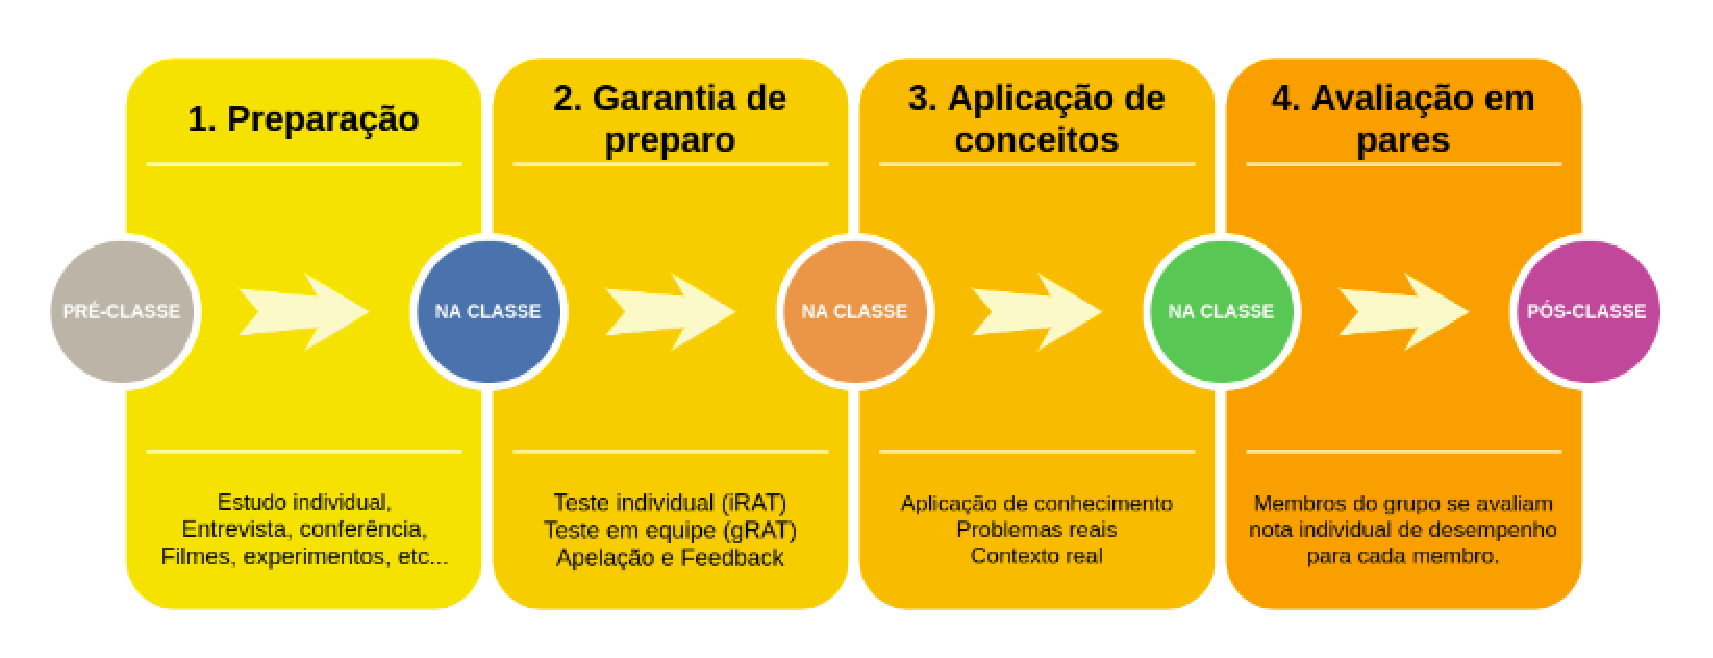
\includegraphics[keepaspectratio=true,scale=0.5]{figuras/tbl2.eps}
  \caption{Etapas do TBL.}
	\label{fig:tbl2}
\end{figure}

\subsection{Detalhando cada etapa do TBL}

\subsubsection{Etapa 1: Preparação individual pré-classe}

Os alunos devem ser responsáveis por se prepararem individualmente para as etapas seguintes do TBL. Se os alunos não se prepararem eles não serão capazes de contribuir para o desempenho de sua equipe. A falta desta preparação dificulta o desenvolvimento de coesão do grupo e resulta em ressentimento por parte da equipe que se preparou (Michaelsen, citado por \citeauthor{bollela}, \citeyear{bollela}).

\subsubsection{Etapa 2: Garantía de prontidão}

O RAT: \textit{Readiness assurance test} (Avaliação de garantia de preparo) que deve ser realizado de maneira individual iRAT e depois em grupo gRAT. É o mecanismo básico que garante a responsabilidade individual pela preparação pré-classe, essa etapa equivale a 50 a 90 minutos (Michaelsen, citado por \citeauthor{bollela}, \citeyear{bollela}). É dividido em 4 atividades:

\begin{enumerate}
  \item \textbf{Avaliação iRAT}: Respondido individualmente sem consulta ou qualquer material, consiste em 10 a 20 questões de múltipla escolha contemplando os conceitos mais relevantes das leituras ou das atividades indicadas previamente, cada questão irá ter um número X de alternativas e o aluno poderá distribuir pontos entre as alternativas, por exemplo, se a questão tem 4 alternativas e ele ta em duvida entre a alternativa A e C ele pode distribuir seus 4 pontos em 2 na A e 2 na C, se a resposta correta for a C ele ganha 2 pontos dos 4, a somatória de todos os pontos divididos pelo total de pontos da prova é calculado a nota do aluno nessa avaliação.
  \item \textbf{Avaliação gRAT}: Respondido em grupo sem consultar, os alunos devem discutir as questões e cada membro deve defender e argumentar as razões para sua escolha até o grupo decidir qual é a melhor resposta, exercitando suas habilidades de comunicação, argumentação e convencimento. Consiste das mesmas questões do iRAT, terá feedbacks imediatos da resposta certa, porém, ele pode ir raspando até acertar, se acertar de primeira recebe pontuação total, 4 se for o número de alternativas existentes, a resposta, porém, a cada erro a pontuação da questão cai pela metade se ele raspar todas as alternativas terão nota zero na questão, o somatório de todos os pontos divididos pelo total é calculado a nota do grupo nessa avaliação.
  \item \textbf{Apelação}: Após as avaliações as equipes podem recorrer a apelação no caso de não concordar com a resposta indicada como correta, todo apelo deve ser feito acompanhado de argumentação, sugestão de melhoria e com consulta a fontes bibliográficas pertinentes. A equipe deve também propor o novo formato e a resposta correta da questão. As equipes que tiverem seus apelos acatados, ganham pontos e o professor tanto pode fazer seu julgamento naquele momento ou então realizar a devolutiva no próximo encontro.
  \item \textbf{Feedback pelo professor}: Assim que as etapas acima se concluir o professor, buscando clarear conceitos fundamentais, oferece feedback a todos simultaneamente, de acordo com as questões que mais gerou dificuldade nas equipes e nos alunos. Ao final desta etapa, os estudantes devem estar confiantes a respeito dos conceitos fundamentais e poderão aplicá-los para resolver problemas mais complexos que serão oferecidos na etapa de aplicação do conhecimento, que se segue numa atividade de TBL.
\end{enumerate}

\subsubsection{Etapa 3: Aplicação de conceitos}

Aplicação do conhecimento (conceitos) adquiridos por meio da resolução de situações problemas ou cenários relevantes e presentes na prática profissional diária do estudante, ou seja, problemas reais que ele pode enfrentar, preparando-os para o que o mercado cobra, deve ocupar a maior parte da carga horária, entre 50 a 90 minutos. O fundamental é que todas as equipes estejam preparadas para argumentar sobre a escolha que fizeram. Conclui-se, assim, um módulo ou unidade educacional em TBL (Michaelsen, citado por \citeauthor{bollela}, \citeyear{bollela}).

\subsubsection{Etapa 4: Avaliação dos estudantes no TBL?}

De acordo com \cite{bollela} os alunos são avaliados pelo seu desempenho individual e também pelo resultado do trabalho em grupo, além de se submeterem à avaliação entre os pares, o que incrementa a responsabilização. A avaliação pelos pares é essencial, pois, os componentes da equipe são, normalmente, os únicos que têm informações suficientes para avaliar com precisão a contribuição do outro

A avaliação em pares, cada integrante da equipe avaliará os outros integrantes da equipe, será disponibilizado uma pontuação máxima para cada membro distribuir entre os outros membros e um campo para dizer o porquê da pontuação podendo inserir feedback para o colega, essa avaliação não precisa se identificar ela é anônima e a pontuação fará parte da nota individual de cada membro da equipe.

Por exemplo, tem cinco membros na equipe, então cada membro terá cem pontos para distribuir aos outros membros, logo pode dar cinquenta pontos para cada se todos trabalharam de forma igual ou se um membro trabalhou menos, insira menos pontos a ele e mais pontos para o que trabalhou mais, no final soma-se os pontos de cada membro e se der o total o membro ganha nota máxima, e se tiver menos pontos que o total ganha a nota proporcional à pontuação.

\subsection{Preparo de um módulo em TBL?}

De acordo com \cite{bollela}, três mudanças são necessárias quando se modifica a estratégia pedagógica de uma aula expositiva, centrada no professor, para uma atividade do tipo TBL, centrada no estudante:

\begin{itemize}
  \item Os objetivos primários devem ser trabalhados apenas com conceitos chaves para objetivos que incluem a compreensão de como estes conceitos devem ser aplicados em situações reais.
  \item O professor passa de alguém que oferece informações e conceitos, para alguém que facilita o aprendizado, ou seja, ele entrega a responsabilidade de gerar conhecimento para o aluno.
  \item É necessária uma mudança no papel e função dos estudantes, que saem da posição de receptores passivos da informação para responsáveis pela aquisição do conhecimento e membros integrantes de uma equipe que trabalha de forma colaborativa para compreender como aplicar o conteúdo na solução de problemas realísticos e contextualizados.
\end{itemize}

Segundo \cite{bollela} uma atividade inicial de treinamento usando o TBL com os alunos deve ser preparada para a primeira aproximação dos estudantes com a metodologia.
